\documentclass[a4paper, 14pt]{extarticle}

% Поддержка языков
\usepackage[english, russian]{babel} 

% Настройка кодировок
\usepackage[T2A]{fontenc}
\usepackage[utf8]{inputenc}

% Настройка шрифтов
\usepackage{fontspec}
\setmainfont[Ligatures=TeX]{Times New Roman} % Шрифт для основного текста документа
\setsansfont[Ligatures=TeX]{Arial}
\setmonofont{Consolas} % Шрифт для кода

\usepackage{tocloft}

% Настройка отступов от краев страницы
\usepackage[left=3cm, right=1.5cm, top=2cm, bottom=2cm]{geometry}

\usepackage{titleps} % Колонтитулы
\usepackage{subfig} % Для подписей к рисункам и таблицам
\usepackage{graphicx} % для вставки картинок
\graphicspath{{./img/}} % Путь до папки с изображениями
% Пакет для отрисовки графиков
\usepackage{tikz}
\usetikzlibrary{arrows,positioning,shadows}
\usepackage{stmaryrd} % Стрелки в формулах
\usepackage{indentfirst} % Красная строка после заголовка
\usepackage{hhline} % Улучшенные горизонтальные линии в таблицах
\usepackage{multirow} % Ячейки в несколько строчек в таблицах
\usepackage{longtable} % Многостраничные таблицы
\usepackage{paralist,array} % Список внутри таблицы
\usepackage[normalem]{ulem}  % Зачеркнутый текст
\usepackage{upgreek, tipa} % Красивые греческие буквы
\usepackage{amsmath, amsfonts, amssymb, amsthm, mathtools} % ams пакеты для математики, табуляции
\usepackage{nicematrix} % Особые матрицы pNiceArray

\linespread{1.5} % Межстрочный интервал
\setlength{\parindent}{1.25cm} % Табуляция
\setlength{\parskip}{0cm}

% Пакет для красивого выделения кода
\usepackage{minted}
\setminted{fontsize=\footnotesize}

% Настройка оглавления
\renewcommand{\contentsname}{Содержание}
\renewcommand{\cftsecleader}{\cftdotfill{\cftdotsep}} % точки между главой и номером
% Добавляем гипертекстовое оглавление в PDF
\usepackage[
bookmarks=true, colorlinks=true, unicode=true,
urlcolor=black,linkcolor=black, anchorcolor=black,
citecolor=black, menucolor=black, filecolor=black,
]{hyperref}

% Убрать переносы слов
\tolerance=1
\emergencystretch=\maxdimen
\hyphenpenalty=10000
\hbadness=10000

\newpagestyle{main}{
	% Верхний колонтитул
	\setheadrule{0cm} % Размер линии отделяющей колонтитул от страницы
	\sethead{}{}{} % Содержание {слева}{по центру}{справа}
	% Нижний колонтитул
	\setfootrule{0cm} % Размер линии отделяющей колонтитул от страницы
	\setfoot{}{\thepage}{} % Содержание {слева}{по центру}{справа}
}
\pagestyle{main}
\pagenumbering{arabic}

% НОВЫЕ КОМАНДЫ
\newcommand{\deriv}[2]{\frac{\partial #1}{\partial #2}}
\newcommand{\n}{\par}
\newcommand{\percent}{\mathbin{\%}}

% Заменяем Рис. на Рисунок
\addto\captionsrussian{\renewcommand{\figurename}{Рисунок}}

% Изменение формата подписей
% Стиль номера таблицы/рисунка #1-Таблица/Рис. #2-номер
\DeclareCaptionLabelFormat{custom}
{%
	#1 #2
}
% Стиль разделителя номера таблици/рисунка и названия таблицы/рисунка
\DeclareCaptionLabelSeparator{custom}{$-$}
% Стиль формата #1-номер таблицы/рисунка #2-разделитель #3-название
\DeclareCaptionFormat{custom}
{%
	#1 #2 #3
}

\captionsetup
{
	format=custom,%
	labelsep=custom,
	labelformat=custom
}

% ПЕРЕГРУЗКА УЖЕ СУЩЕСТВУЮЩИХ КОМАНД
\renewcommand{\epsilon}{\varepsilon} % Заменить знак эпсилон
\renewcommand{\phi}{\varphi}
\renewcommand{\kappa}{\varkappa}
\renewcommand{\lambda}{\uplambda}


\begin{document}
	\newcommand{\Faculty}{Факультет программной инженерии и компьютерной техники}

\newcommand{\TeacherPosition}{}
\newcommand{\TeacherName}{Белокон Юлия Алексеевна}

\newcommand{\LabSubject}{Информатика}
\newcommand{\LabNumber}{\textnumero 6}
\newcommand{\LabName}{Работа с системой компьютерной вёрстки \TeX}
\newcommand{\Variant}{60}

\newcommand{\StudentGroup}{Р3115}
\newcommand{\StudentName}{Разыграев Кирилл Сергеевич}


\thispagestyle{empty}

\begin{figure}[h]
	\centering
	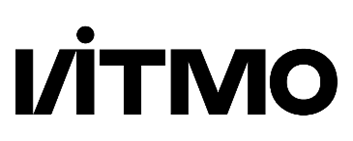
\includegraphics{logo}
\end{figure}
\vspace{-\baselineskip}


\begin{center}
	Федеральное государственное автономное образовательное \\
	учреждение высшего образования\\
	«Национальный исследовательский университет ИТМО»
\end{center}\par

\begin{center}
	\vspace{12pt}
	\Faculty
\end{center}\par

\vspace{\fill}
\begin{center}
	Лабораторная работа \LabNumber \\
	По дисципление: \LabSubject \\
	Тема: <<\LabName>> \\
	Вариант \Variant
\end{center}\par

\vspace{\fill}
\vbox{
	\hfill
	\vbox{
		\hbox{\textbf{Выполнил:} \StudentName}
		\hbox{\textbf{Группа:} \StudentGroup \\}
		\hbox{\textbf{Преподаватель:} \TeacherPosition \TeacherName}
	}
} 


\vspace{\fill}
\begin{center}
	Санкт-Петербург, \the\year{}
\end{center}\par

\newpage

	
	\tableofcontents
	\newpage
	
	\section*{Задание}
	\addcontentsline{toc}{section}{Задание}
	\begin{enumerate}
	\item Создать приведенное в варианте дерево каталогов и файлов с содержимым. В качестве корня дерева использовать каталог lab0 своего домашнего каталога. Для создания и навигации по дереву использовать команды: mkdir, echo, cat, touch, ls, pwd, cd, more, cp, rm, rmdir, mv.
	\begin{figure}[h]
		\centering
		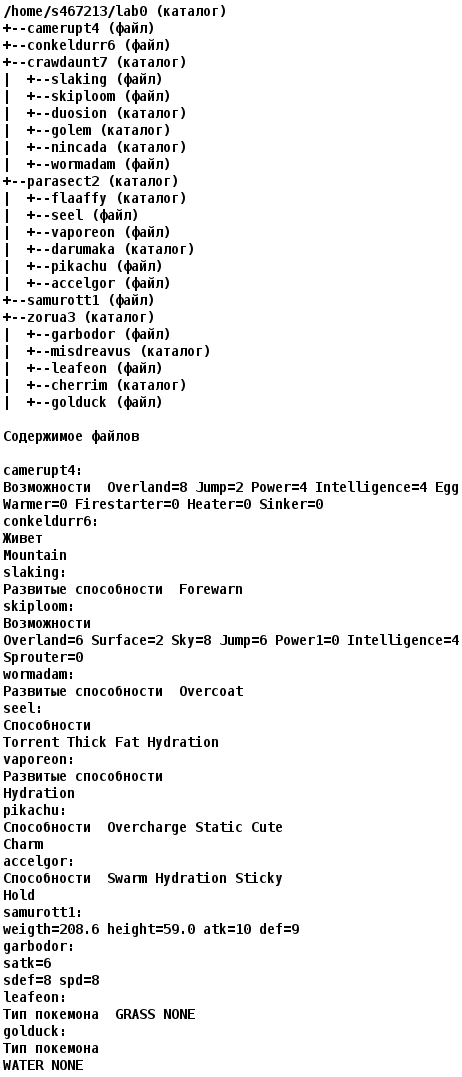
\includegraphics[scale=0.5]{task}
	\end{figure}
	
	\item Установить согласно заданию права на файлы и каталоги при помощи команды chmod, используя различные способы указания прав.
	\begin{itemize}
		\item camerupt4: владелец должен не иметь никаких прав; группа-владелец должна не иметь никаких прав; остальные пользователи должны читать файл
		 \item conkeldurr6: владелец должен читать и записывать файл; группа-владелец должна записывать файл; остальные пользователи должны записывать файл
		 \item crawdaunt7: -wxrwxr-x
		 \item slaking: владелец должен не иметь никаких прав; группа-владелец должна читать и записывать файл; остальные пользователи должны записывать файл
		 \item skiploom: владелец должен не иметь никаких прав; группа-владелец должна читать файл; остальные пользователи должны читать и записывать файл
		 \item duosion: права 555
		 \item golem: права 337
		 \item nincada: права 555
		 \item wormadam: ------rw-
		 \item parasect2: -wx-wxr-x
		 \item flaaffy: rwxr-x-w-
		 \item seel: владелец должен читать и записывать файл; группа-владелец должна читать файл; остальные пользователи должны не иметь никаких прав
		 \item vaporeon: владелец должен читать файл; группа-владелец должна читать файл; остальные пользователи должны не иметь никаких прав
		 \item darumaka: владелец должен читать, записывать директорию и переходить в нее; группа-владелец должна читать директорию и переходить в нее; остальные пользователи должны записывать директорию
		 \item pikachu: владелец должен не иметь никаких прав; группа-владелец должна читать файл; остальные пользователи должны читать и записывать файл
		 \item accelgor: права 044
		 \item samurott1: r--------
		 \item zorua3: r-x--x-wx
		 \item garbodor: владелец должен читать и записывать файл; группа-владелец должна не иметь никаких прав; остальные пользователи должны не иметь никаких прав
		 \item misdreavus: владелец должен читать директорию и переходить в нее; группа-владелец должна только переходить в директорию; остальные пользователи должны записывать директорию и переходить в нее
		 \item leafeon: r-----r--
		 \item cherrim: владелец должен читать директорию и переходить в нее; группа-владелец должна читать, записывать директорию и переходить в нее; остальные пользователи должны читать, записывать директорию и переходить в нее
		 \item golduck: права 640
	\end{itemize}
	
	\item Скопировать часть дерева и создать ссылки внутри дерева согласно заданию при помощи команд cp и ln, а также комманды cat и перенаправления ввода-вывода.
	\begin{itemize}
		\item скопировать рекурсивно директорию parasect2 в директорию lab0/crawdaunt7/nincada
		\item скопировать файл camerupt4 в директорию lab0/crawdaunt7/duosion
		\item cоздать жесткую ссылку для файла conkeldurr6 с именем lab0/crawdaunt7/slakingconkeldurr
		\item создать символическую ссылку c именем Copy\_5 на директорию zorua3 в каталоге lab0
		\item объеденить содержимое файлов lab0/zorua3/golduck, lab0/parasect2/accelgor, в новый файл lab0/camerupt4\_76
		\item скопировать содержимое файла conkeldurr6 в новый файл lab0/parasect2/accelgorconkeldurr
		\item cоздать символическую ссылку для файла camerupt4 с именем lab0/crawdaunt7/slakingcamerupt
	\end{itemize}
	
	\item Используя команды cat, wc, ls, head, tail, echo, sort, grep выполнить в соответствии с вариантом задания поиск и фильтрацию файлов, каталогов и содержащихся в них данных.
	\begin{itemize}
		\item Рекурсивно подсчитать количество символов содержимого файлов из директории lab0, имя которых начинается на 'c', результат записать в файл в директории /tmp, подавить вывод ошибок доступа
		\item Вывести четыре первых элемента рекурсивного списка имен и атрибутов файлов в директории lab0, содержащих строку "da", список отсортировать по убыванию даты модификации файла, подавить вывод ошибок доступа
		\item Рекурсивно вывести содержимое файлов из директории lab0, имя которых заканчивается на 'r', строки отсортировать по имени a->z, ошибки доступа перенаправить в файл в директории /tmp
		\item Вывести содержимое файлов: wormadam, seel, vaporeon, pikachu, accelgor, garbodor, leafeon, исключить строки, заканчивающиеся на 'n', регистр символов игнорировать, добавить вывод ошибок доступа в стандартный поток вывода
		\item Подсчитать количество символов содержимого файлов в директории crawdaunt7, результат записать в файл в директории /tmp, добавить вывод ошибок доступа в стандартный поток вывода
		\item Вывести два первых элемента рекурсивного списка имен и атрибутов файлов в директории lab0, содержащих строку "ldu", список отсортировать по возрастанию даты изменения записи о файле, ошибки доступа перенаправить в файл в директории /tmp
	\end{itemize}
	
	\item Выполнить удаление файлов и каталогов при помощи команд rm и rmdir согласно варианту задания.
	\begin{itemize}
		\item Удалить файл conkeldurr6
		\item Удалить файл lab0/crawdaunt7/wormadam
		\item удалить символические ссылки lab0/crawdaunt7/slakingcameru*
		\item удалить жесткие ссылки lab0/crawdaunt7/slakingconkeldu*
		\item Удалить директорию zorua3
		\item Удалить директорию lab0/parasect2/flaaffy
	\end{itemize}
\end{enumerate}
	
	\section*{UML - диаграмма}
	\addcontentsline{toc}{section}{UML - диаграмма}
	\begin{figure}[h]
		\centering
		\hspace*{-2cm}
		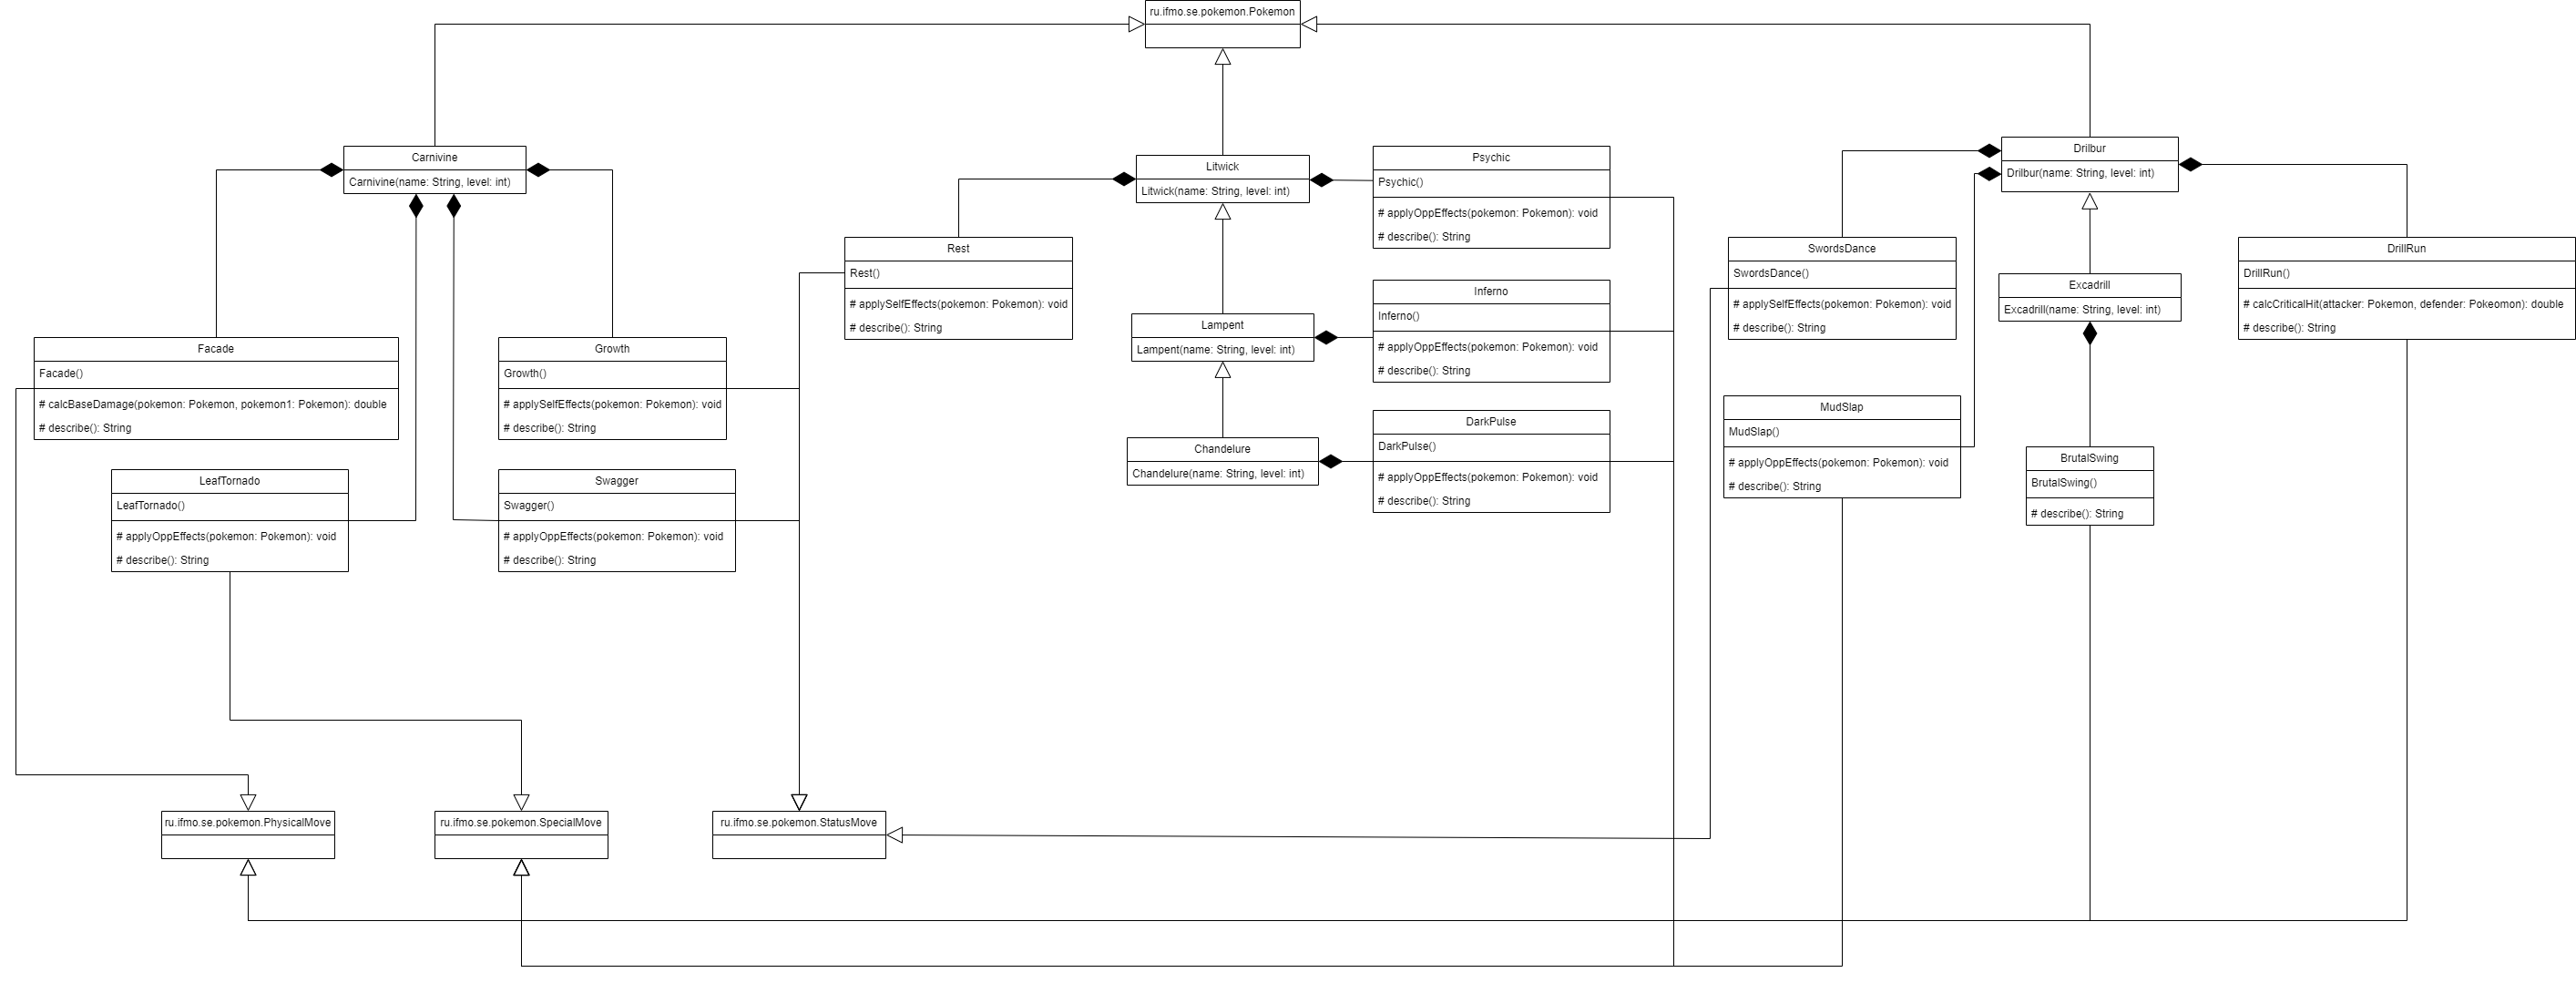
\includegraphics[scale=0.19]{uml}
	\end{figure}
	
	\section*{Исходный код программы}
	\addcontentsline{toc}{section}{Исходный код программы}
	\url{https://github.com/lysmux/itmo/tree/proga/proga/1_semestr/labs/lab2_pockemons}
	
	\section*{Результат работы программы}
	\addcontentsline{toc}{section}{Результат работы программы}
	\url{https://github.com/lysmux/itmo/blob/proga/proga/1_semestr/labs/lab2_pockemons/docs/output.log}
	
	\section*{Вывод}
	\addcontentsline{toc}{section}{Вывод}
	В процессе выполнения работы я:
\begin{itemize}
	\item познакомился с основами ООП в Java
	\item научился подключать сторонние .jar  библиотеки
	\item познакомился с системой сборки Gradle и научился создавать  fatJar с её помощью
\end{itemize}
	
\end{document}